\documentclass[12pt]{article}
\usepackage{hyperref}
\usepackage{graphicx}
\usepackage{enumerate}
\usepackage{fancyhdr}
\pagestyle{fancy}
\fancyhead{}
\rhead{RTT Estimation}
\lhead{
\includegraphics[scale=0.2]{logo.jpg}}
\setlength{\topmargin}{-.5in}
\setlength{\textheight}{9in}
\setlength{\oddsidemargin}{.125in}
\setlength{\textwidth}{6.25in}

\begin{document}


\title{\underline{RTT  Estimation}}
\author{Anshul Jain\\Y09UC027}
\renewcommand{\today}{November 12, 2011}
\maketitle
\begin{abstract}
\bf Round Trip Time (RTT) \rm is the length of time it takes for a segment to be sent plus the length of time it takes for an acknowledgment of that segment to be received. The RTT basically provides a basis to set the retransmission time in case of packet loss. Our analysis concluded that there are three different RTT estimation mechanisms – \\a) TCP Algorithm \\b) Jacobson’s Algorithm \\c) Karn’s Algorithm.\\Our report shows the practical implementations of these mechanisms and provides its comparative statistics
\end{abstract}
\section{THEORY}
\bf The transport layer \rm  is the heart of the whole protocol hierarchy. Its task is to provide reliable, cost-effective data transport from the sourse machine to the destination machine, independently of the physical networks currently in use.
 
A \bf  port \rm  is associated with an IP address of the host, as well as the type of protocol used for communication. The protocol that primarily use the ports are the Transport Layer protocols, such as the Transmission Control Protocol (TCP). A port is identified for each address and protocol by a 16-bit number, commonly known as the \bf  port number \rm. The port number completes the destination address for a communications session. Thus, different IP addresses or protocols may use the same port number for communication.


\bf Sockets \rm  are interfaces that can  plug into each other over a network  so that the programs connected can communicate.
Internet sockets constitute a mechanism for delivering incoming data packets to the appropriate application process or thread, based on a combination of local and remote IP addresses and port numbers.\\
\newpage
The socket primitives for TCP : 

\begin{center}
\begin{tabular}{ | l | p{10cm} | }
\hline
 \bf Primitive \rm & \bf Meaning \rm \\
\hline SOCKET  & Create a new communication end point. \\
\hline BIND & Attach a local address to the socket. \\
\hline LISTEN & Announce willingness to accept the connections:give queue size. \\
\hline ACCEPT & Block the caller until a connection attempt arrives. \\
\hline CONNECT & Actively attempt to establish a connection. \\
\hline SEND & Send some data over the connection. \\
\hline RECEIVE & Receive some data from the connection. \\
\hline CLOSE & Release the connection. \\
\hline
\end{tabular}
\end{center}
\bf RTT (Round Trip Time) \rm  is the time required for data to go from a source to a destination and then receive acknowledgement of the arrival. The RTT has many applications to TCP. One of the most important is the Retransmission Time-Out (RTO) timer. This timer is maintained with each connection, and if the sender does not receive acknowledgement upon the expiration of the timer, TCP will retransmit the data and restart the timer. This timer is based upon the size of the packet. Because each packet may be a different size, the timer cannot be a fixed value and therefore relies on an accurate estimation of the RTT. Shorter RTT usually indicate smaller service time, i.e. faster transfer rate. RTT in real world traffic is highly correlated with geographical distance.\\
\\ Challenges that affect RTT estimation:
\begin{enumerate}
\item Persistent congestion 
\item Route change
\end{enumerate}
To achieve optimal throughput, short timeout interval should be used. Unfortunately, what is good for throughput is disastrous for efficient network utilization. If the timeout interval is too short then a large number of packets may be retransmitted unnecessarily because the sender times out too soon.\\
\\ We have tried the following three approaches to efficiently estimate the RTT
over the network : 

\subsection{\underline{TCP Algorithm}}

TCP implementations are expected to predict future round trip times by sampling the behavior of datagrams sent over a connection and averaging those samples into a “smoothed” round trip time estimate, SRTT.\\
Every time a new packet is sent, SRTT is updated using the formula:\\
\[
(SRTT)_{new} =  \alpha \times (SRTT)_{prev} + (1-\alpha )\times (RTT)\\
\]

where  $\alpha$  is  the smoothening factor with a recommended value of 0.875 and  RTT  is the latest round trip time measured. $\alpha$ denotes that 87.5 \% of each new estimate is from the  previous SRTT estimate  and 12.5 \% is from the new measurement.\\
 Retransmission Time Out (RTO)  value is set to be :\\

\[
 (RTO )_{new} = \beta  \times  (SRTT)_{new}
\] 
where $\beta$ is the delay variance factor with a recommended value of 2. \\ \\
The accurate measurement of RTTs is difficult when there are retransmissions. Also the algorithm to compute the smoothed round trip time is inadequate, because it incorrectly assumed the variance in RTT values would be small and constant. These problems were solved by Karn’s and Jacobson’s algorithm respectively.
\subsection{\underline{Jacobson's Algorithm}}
Jacobson’s algorithm is a refinement of TCP algorithm that dynamically computes the variance instead of using a fixed $\beta$. The proposal has been to calculate the RTO based on both the mean and variance of RTT rather than just calculating RTO as a constant multiple of mean RTT.\\
Jacobson’s calculation of the RTO depends on both the smoothed RTT and the smoothed deviation, whereas the original method used a multiple of the smoothed RTT.\\
Jacobson’s RTT estimation algorithm is as follows:
\[
Error = RTT  –  (SRTT)_{prev}
\]
\[
(SRTT)_{new} = (SRTT)_{prev} + g \times Error			
\]
\[
D_{new} = h\times (|Error| - D_{prev})
\]
\[
(RTO)_{new} = (SRTT)_{new} + 4\times D_{new}
\]
where SRTT is the smoothed RTT and D is the smoothed mean deviation. Error is the difference between measured value just obtained and the current RTT estimator. Both (SRTT)$_{new}$ and D$_{new}$ are used to calculate the next transmission timeout (RTO$_{new}$). The gain g is for the average and is set to (1/8). The gain for the deviation is h and is set to (1/4). The larger the gain for deviation makes the RTO go up faster when the RTT changes.
\subsection{\underline{Karn's Algorithm}}
When retransmissions occur, TCP cannot know whether the received acknowledgement was issued on the receipt of the first packet or on the receipt of one of the subsequent retransmitted packets. This is called the \bf retransmission ambiguity problem\rm.\\
If the TCP chooses to measure the new RTT, as the interval of time from first transmission to the receipt of the acknowledgement, it runs the risk to inflate unnecessarily the value of RTT estimator. If the TCP chooses to measure the new RTT, as the interval of time from the most recent retransmission to the receipt of acknowledgement, it runs the risk to decrease inappropriately the value of RTT estimator.\\
Karn solved this problem by proposing the following simple rules:
\begin{enumerate}
\item When an acknowledgement arrives for a packet that has been sent more than once, ignore any round trip time measurement based on this packet.
\[
(SRTT)_{new} =  \alpha \times (SRTT)_{prev} + (1-\alpha )\times (RTT)\\
\]
\item Don’t calculate the new RTO, but reuse instead the last backed off RTO for the next transmission. Only when a packet is acknowledged without an intervening retransmission will the RTO be recalculated from the RTT estimator.
\end{enumerate}
\[
(RTO)_{new} = 2\times (RTO)_{prev}
\]
\section{EXPERIMENT}
\subsection{\underline{Experimental Setup}}
The synchronization of server and client was done using the Network Service Provider(NTP) with the time server as 172.22.2.95. The environment was not same when different observations for these algorithms were made.\\ \\
To create real world traffic conditions server and client were made in two different networks, the client on MTNL and the server on Reliance so that the packet is transmitted through many routers in between.


\subsection{\underline{Assumptions}}

During the course of our project the following assumptions have been made :
\begin{enumerate}
\item In Karn’s and TCP algorithm the first RTO has been assumed to be 0.3ms,                         where as in Jacobson’s algorithm it has been assumed to be 100ms.
\item Until the acknowledgement of the sent segment has been received, the next segment is not being sent, thus the packets arrive in order.\\
\end{enumerate}
\section{RESULTS}
In the following graphs, the X-axis represents the packet number of the segment sent and the Y-axis is the time line in milliseconds(ms).\\
Although the observations were made for 1500 packets, the plot for real world traffic is taken only for 500 for better visualization and understanding.
\subsection{\underline{TCP Algorithm}}
\begin{center}
 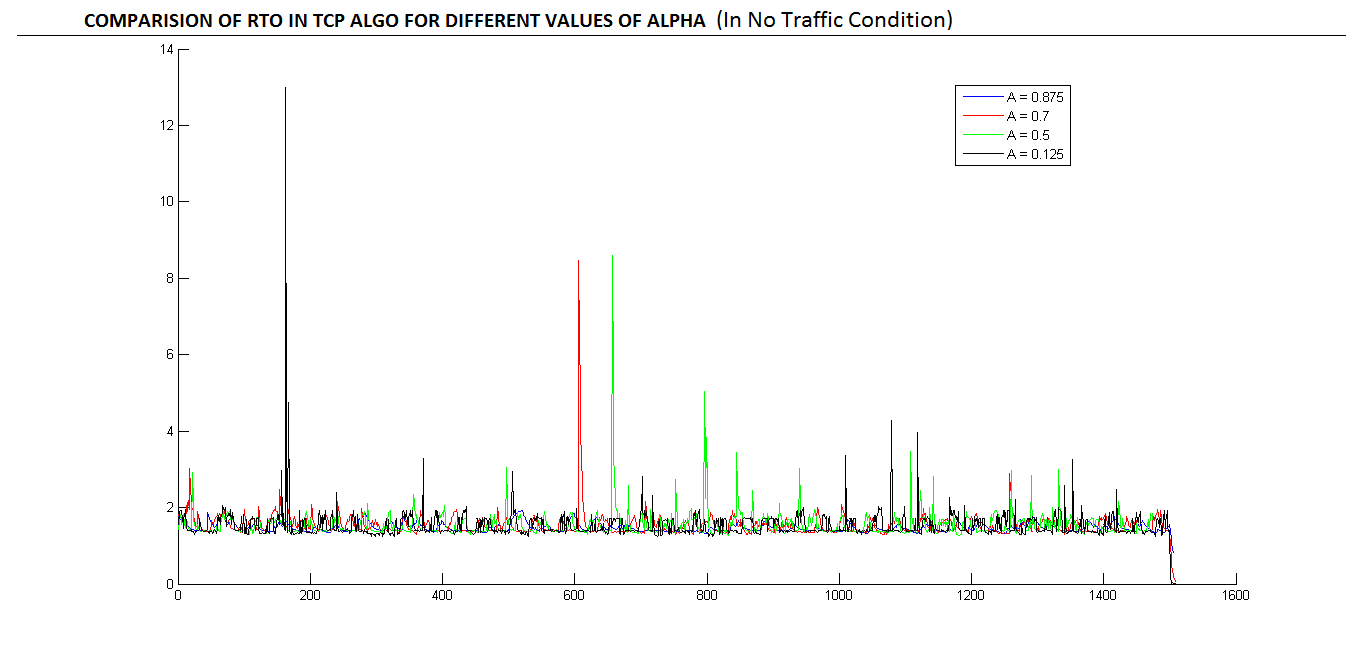
\includegraphics[scale=0.5]{tcp.png}
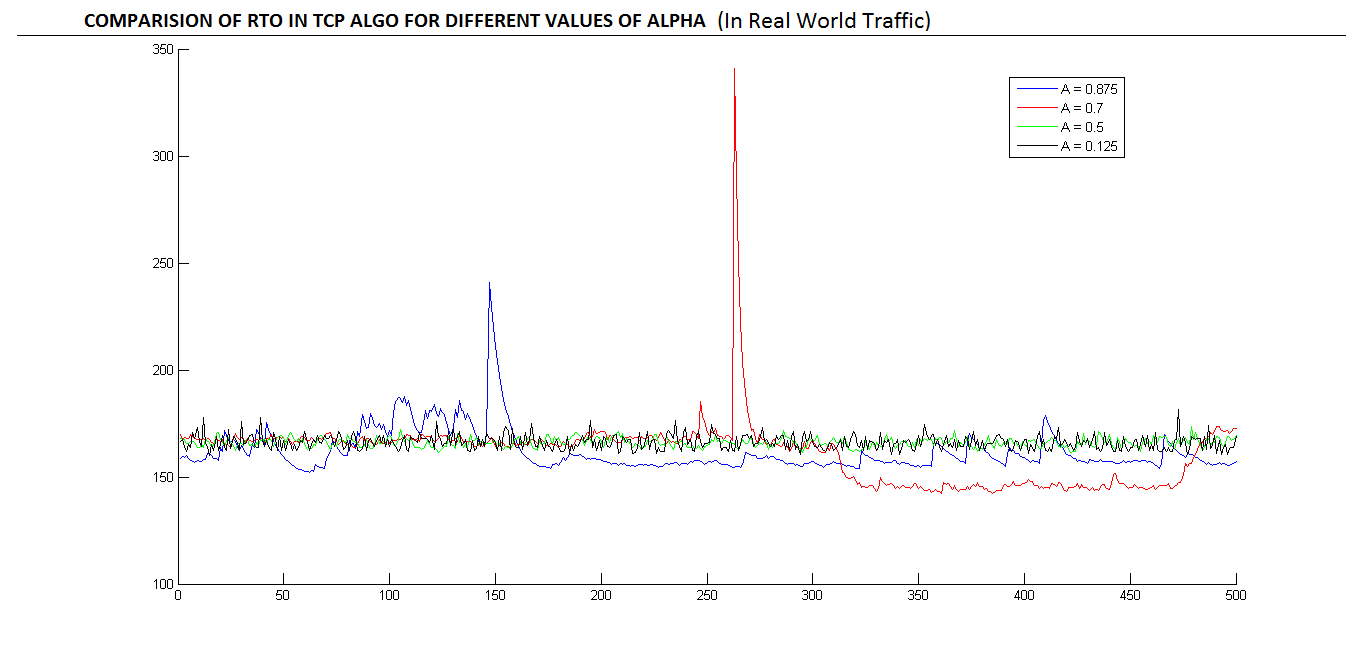
\includegraphics[scale=0.5]{tcp1.png}
\end{center}
From the above graphs it has been observed that :
\begin{enumerate}
\item Higher the value of α, more smoothened is the SRTT wrt the RTT.
\item Lower value of α denotes higher dependence on current measured RTT. So whenever there is a timeout that is there is a sudden increase in RTT, and so there is a peak in the graph of RTO. Thus, lower the $\alpha$ higher will the peak value.
\end{enumerate} 
\subsection{\underline{Jacobson's Algorithm}}
\begin{center}
 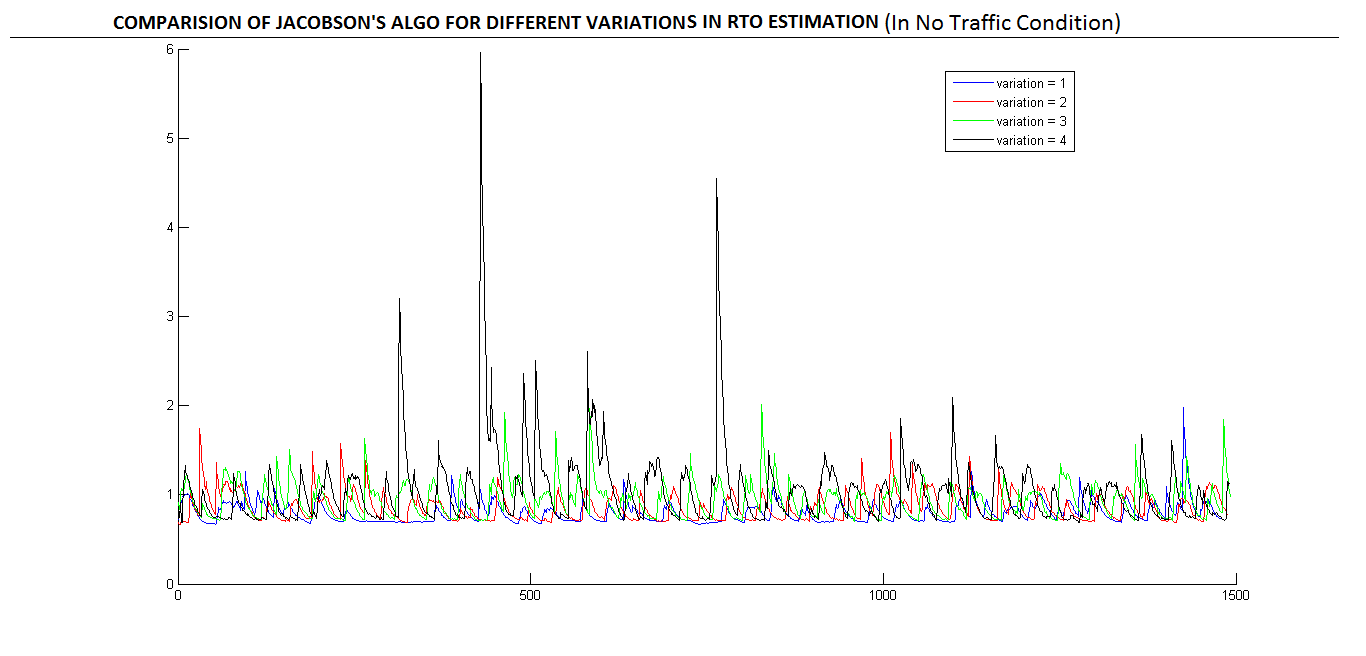
\includegraphics[scale=0.5]{jacob.png}
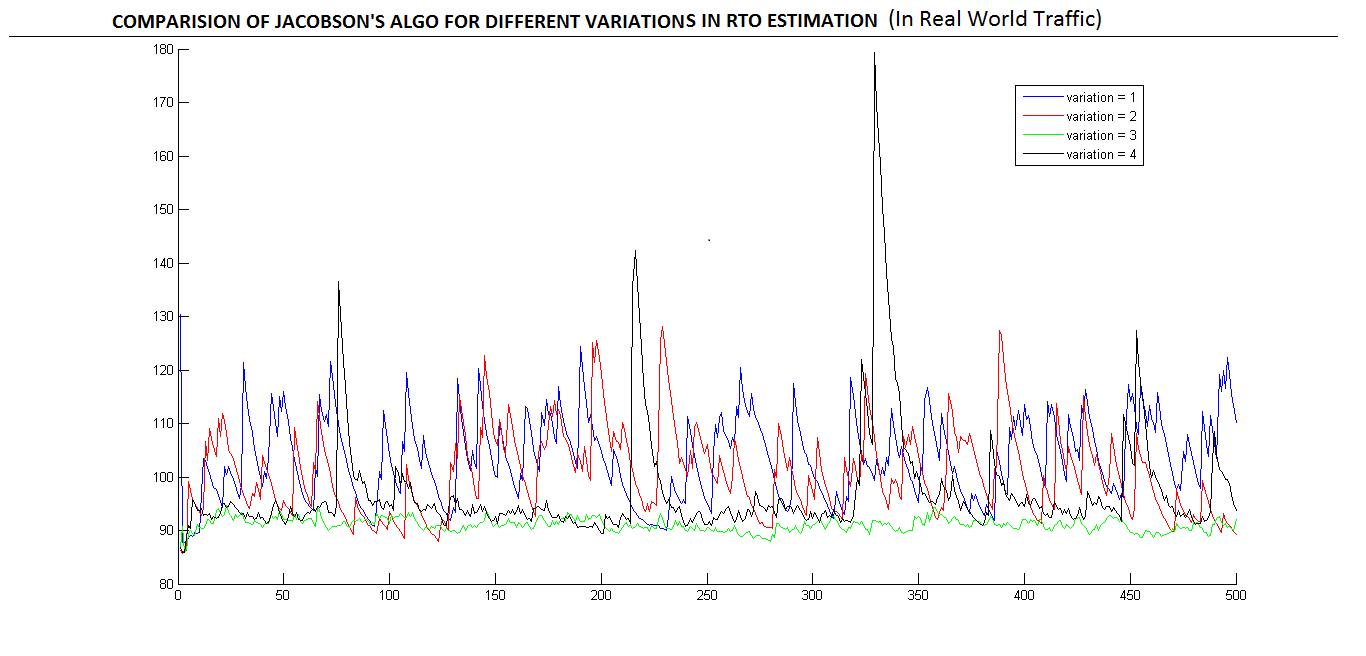
\includegraphics[scale=0.5]{jacob1.png}
\end{center}
From the above graph, we can infer that:
\begin{enumerate}
\item Lower value of variation denotes lower dependence on current measured RTT. Thus, higher the variation higher will the peak value. Hence it is observed that for variation = 4, peak value is highest.
\item We know that RTO is inversely proportional to throughput and lower the number of retransmissions better is the network utilization. So considering both the factors, variation =3 provides the best result.
\end{enumerate}
\subsection{\underline{Karn's Algorithm}}
\begin{center}
 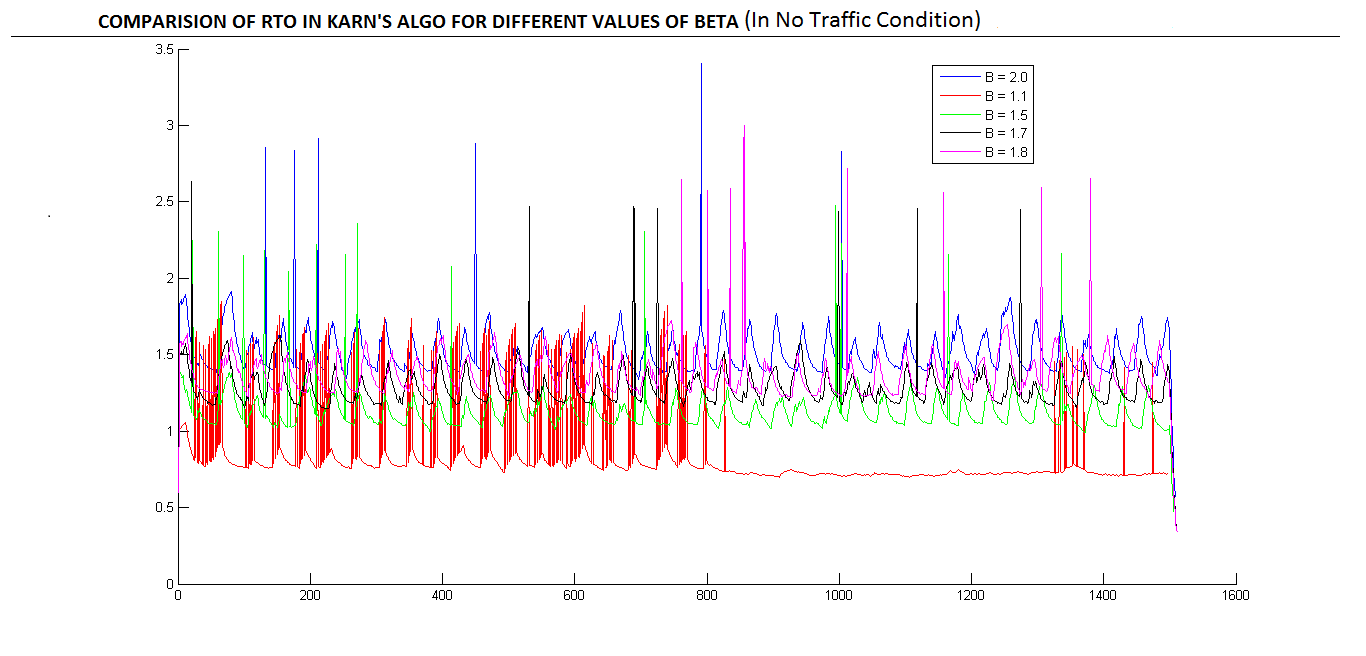
\includegraphics[scale=0.5]{karn.png}
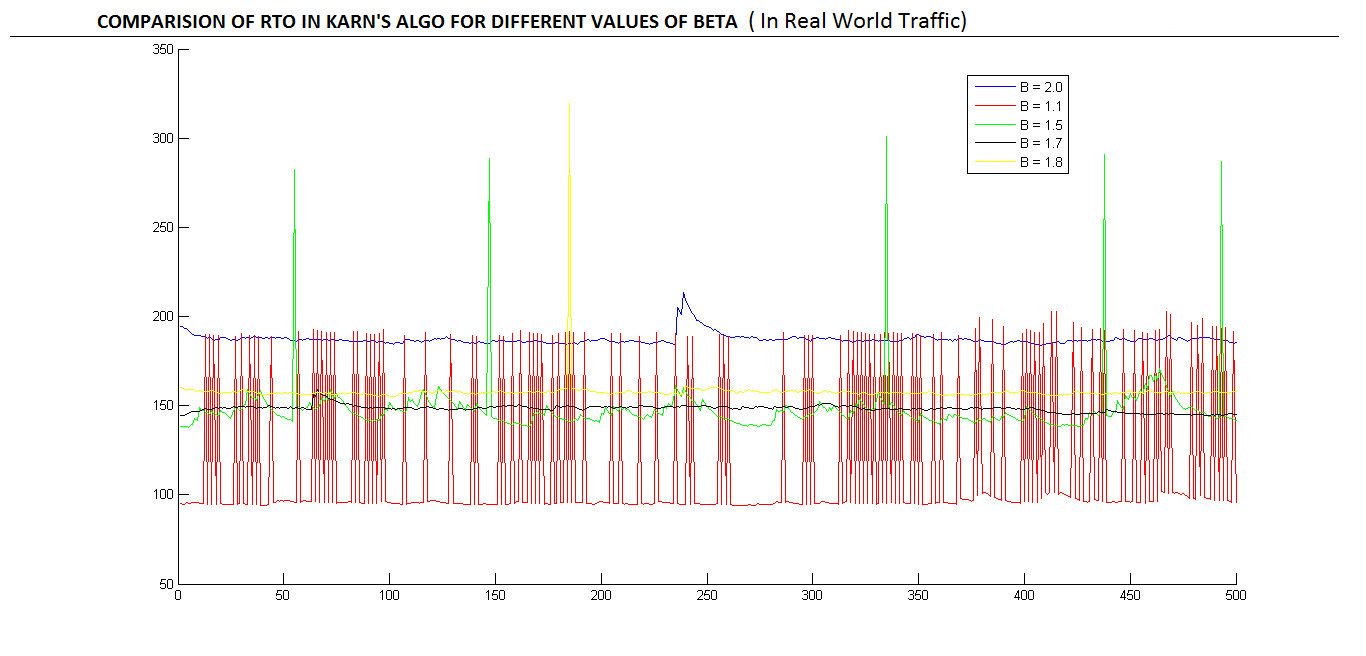
\includegraphics[scale=0.5]{karn1.png}
\end{center}
From the above graph it can be said that, considering the network utilization we only take into account the cases for which sudden peaks(retransmissions) are less. And considering the throughput the case for which RTO is lower provides the better result. Hence $\beta$=1.7 is best.
\subsection{\underline{Comparison between the three algorithms}}
\begin{center}
 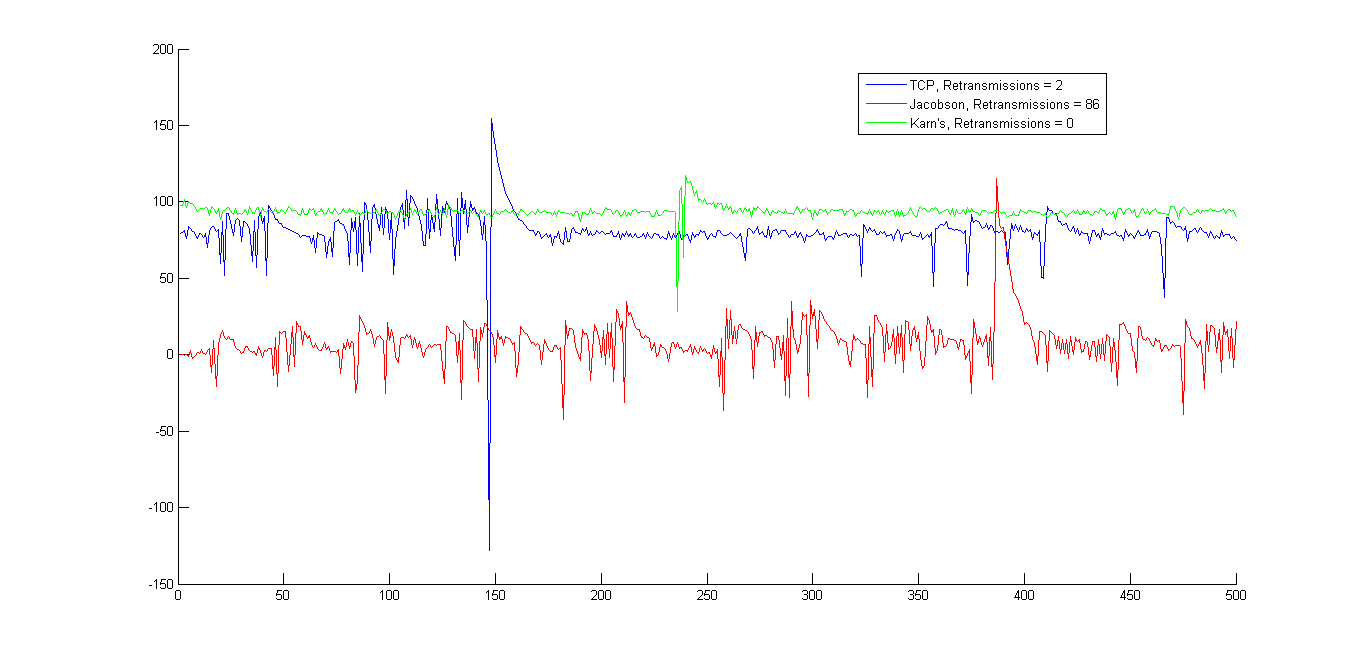
\includegraphics[scale=0.5]{algocmp.png}
\end{center}
\begin{center}
X-axis $\rightarrow$ Packet Number\\
Y-axis $\rightarrow$ (RTO - RTT) in ms
\end{center}
Whenever the graph goes below the X-axis, the value of RTO is less than RTT. This denotes there is a TIMEOUT and hence retransmission. From the graph, the throughput for Jacobson’s algorithm comes out to be the best. But, it has a lot of retransmissions, so the network utilization is VERY POOR.\\ \\
So, now taking throughput as parameter, TCP Algorithm is better while in terms of network utilization Karn’s Algorithm provides better results.   

\section{SHORTCOMINGS}
\begin{enumerate}
\item IP address of the sender should be known.
\item The time used is the epoch time i.e. the number of seconds that have elapsed since  January 1, 1970.
\item The first RTO is being assumed, therefore the first packet is getting timeout in most of the cases and is being retransmitted.
\item More than one client cannot be connected to the server simultaneously as it gives connect error.
\item Although the number of iterations in server and client are 1500 we are not getting our output corresponding to 1500 iterations because the client runs for 1500 times where as the server increases the count of iteration whenever there is a retransmission and hence our loop in server is running for more than 1500 times and the client closes its connection with the server as soon as it finishes it 1500 iterations. But the number of packets sent are still 1500.
\end{enumerate}
\section{PROBLEMS FACED}
\begin{enumerate}
\item Two sockets could not be opened due to bind error.
\item We were trying to send to the client the packet number as the data but it could not be implemented so instead we have to send a static message.
\item Although the two machines could not be synchronized upto the microseconds precision we could efficiently estimate the RTT as RTT estimation is independent of time synchronization between two machines.

\end{enumerate}
\section{CONCLUSIONS}
RTT could be estimated correctly and hence an efficient retransmission timeout could be obtained. There is always a tradeoff between network utilization and throughput. 

\section{REFERENCES}
\begin{enumerate}
\item \url{http://surf-it.soe.ucsc.edu/sites/default/files/lukin_surfit10_report.pdf}
\item \url{http://www.ietf.org/rfc/rfc2988.txt}
\item \url{https://docs.google.com/viewer?a=v&q=cache:LFf-mE9SlIJ:citeseerx.ist.psu.edu/viewdoc/download\%3Fdoi\%3D10.1.1.122.7350\%26rep\%3Drep1\%26type\%3Dpdf+c+code+implementation+of+round+trip+time+algorithm\&hl=en\&gl=in\&pid=bl\&srcid=ADGEESh_J3xzQmI1W3rimEVVnZ-8jGseX0lhiNwgwsWhWflxELQ9RoYCaDq610eYrbf4gG47LIQ9uMO2KwZLWpbJxl9tdFETvr6cdEIQ24yAVElqXs9MVX7bHRyy6Ik1QPTtcskUpYMs\&sig=AHIEtbQbUC1JEGDBZljeW1JQ-ZzMYVxWlw}
\item \url{http://www.icao.int/anb/Panels/ACP/ATNP/Meetings/wg2/wps/w2wp512.pdf}
\item 	\bf Computer Networks by Andrew S. Tanenbaum. \rm
\end{enumerate}
\end{document}
